\documentclass{article}

\usepackage{graphicx} % Required for inserting images
\usepackage{array}
\usepackage{amsmath}
\usepackage{blindtext}
\usepackage{titlesec}

\setlength{\parindent}{0in}
\setlength{\oddsidemargin}{0in}
\setlength{\textwidth}{6.5in}
\setlength{\textheight}{8.8in}
\setlength{\topmargin}{0in}
\setlength{\headheight}{18pt}

\title{CheatSheet INF102}
\author{Erik Fjelltveit Nyhuus}
\date{November 2024}

\begin{document}
\maketitle

\tableofcontents

\newpage

% Add binary search algorithm, the two variants. Recurrsion and iterative.
% List of the different sorting algorithems and there sudocode. There usecaese. 
% How to use Collections.sort() Comparator, Comparable.
% Quickselect, better understanding. 
% Exapmle code.
% Priorityqueue, how does it work, where should you use it. What are the implementations.
% Added usefull code from labs to download. 

\section{Sorting Algorithms}
\subsection{Selection sort}
Time Complexity = $O(n^2)$\\
Sorts an array by repeatedly selecting the smallest or largest element from the unsorted portion
and swapping it with the first unsorted element. Continues until list is sorted.
\subsection{Insertion sort}
Time Complexity = $O(n^2)$\\
Simple sorting algorithm that works by iteratively inserting each element of an unsorted list into its correct 
position in a sorted portion of the list. The same algorithm you use when sorting playing cards. 
You pick a card and insert it into the correct relative position. 
\subsection{Bubble sort}
Time Complexity = $O(n^2)$\\
Works by repeatedly swapping the adjacent elements if they are in the wrong order. Continues 
this process until it has a pass with know swaps.
\subsection{Quick sort}
Worst Case = $O(n^2)$ Occures with poor pivot.\\ 
Average Case = $\theta(nlog(n))$\\
Based on divide and conquer. Quick sort chooses a random pivot P, and swaps P with the last element. Two pointer, left bound and right bound points to index 0 and n - 1.
Left bound moves to the right until it hits an element $\geq P$ or crosses the right bound. Right bound does the samle until i finds an element $\leq P$. 
Swap elements that right and left bound points to. Continue this process until either they crosses, this indicates that all elements smaler than $P$ is on the left and larger are one the right.
The last element right or left bound points to swap places with pivot. Since pivot was left at the end in first step. 
Repeat this with left and right sub-list.  
\subsection{Merge sort}
Average Case = $(nlog(n))$\\
Divide the list into two smaller sublists, continues on dividing until list has size 1. Merges each of the smaller lists in correct order until everything is sorted. 
\subsection{Bucket sort}
Average Case = $(nlog(n))$\\
Works if you have repeated elements in a list. Adds elements into different groups based on size. Sort each bucket on it own afterwards. 

\subsection{Radix sort}
Rather than comparing elements directly, Radix Sort distributes the elements into buckets based on each digit’s value. 
By repeatedly sorting the elements by their significant digits, from the least significant to the most significant.

\newpage

\section{ArrayList vs. LinkedList}
\begin{table}[!ht]
\centering
\begin{tabular}{|l|c|c|}
\hline
\textbf{Operation} & \textbf{ArrayList} & \textbf{LinkedList} \\
\hline
size() & O(1) & O(1) \\
\hline
add() & O(n)* & O(1) \\
\hline
contains(obj) & O(n) & O(n) \\
\hline
remove(obj) & O(n) & O(n) \\
\hline
toArray() & O(n) & O(n) \\
\hline
indexOf(obj) & O(n) & O(n) \\
\hline
get(int i) & O(1) & O(n) \\
\hline
set(int i, E e) & O(1) & O(n) \\
\hline
addFirst() & O(n) & O(1) \\
\hline
\end{tabular}
\end{table}
\begin{itemize}
  \item *O(1) in amortized time (when resizing is not needed)
\end{itemize}


\section{ArrayList vs. LinkedList (Queue/Stack)}
\begin{table}[!ht]
\centering
\begin{tabular}{|l|c|c|c|c|}
\hline
& \textbf{ArrayList} & & \textbf{LinkedList} & \\
\hline
& \textbf{Queue} & \textbf{Stack} & \textbf{Queue} & \textbf{Stack} \\
\hline
offer / push & O(n) & O(n)* & O(1) & O(1) \\
\hline
poll / pop & O(1) & O(1) & O(1) & O(1) \\
\hline
peek & O(1) & O(1) & O(1) & O(1) \\
\hline
\end{tabular}
\end{table}
\begin{itemize}
  \item *O(1) in amortized time (when resizing is not needed)
\end{itemize}

\section{PriorityQueue}

\subsection{PriorityQueue}
\begin{table}[!ht]
  \centering
  \begin{tabular}{|l|c|}
  \hline
  \textbf{Operation} & \textbf{Time Complexity} \\
  \hline
  add() & O(log(n))\\
  \hline
  remove(Head) & O(log(n))\\
  \hline
  remove(Specific object) & O(n)\\
  \hline
  poll() & O(log(n))\\
  \hline  
  peek() & O(1)\\
  \hline  
  size() & O(1)\\
  \hline  
  \end{tabular}
  \end{table}

\subsection{PriorityQueue - SortedList}
\begin{table}[!ht]
\centering
\begin{tabular}{|l|c|}
\hline
\textbf{Operation} & \textbf{Time Complexity} \\
\hline
add(T element) & O(n) \\
\hline
T findMin() & O(1) \\
\hline
T removeMin() & O(1) \\
\hline
\end{tabular}
\end{table}
\subsection{PriorityQueue - LinkedList}
\begin{table}[!ht]
\centering
\begin{tabular}{|l|c|}
\hline
\textbf{Operation} & \textbf{Time Complexity} \\
\hline
add(T element) & O(1) \\
\hline
T findMin() & O(n) \\
\hline
T removeMin() & O(n) \\
\hline
\end{tabular}
\end{table}

\newpage


\section{HashSet vs. TreeSet}
\begin{table}[!ht]
\centering
\begin{tabular}{|l|c|c|}
\hline
\textbf{Operation} & \textbf{HashSet} & \textbf{TreeSet} \\
\hline
add() & O(1)* & O(log(n)) \\
\hline
remove() & O(1)* & O(log(n)) \\
\hline
contains(obj) & O(1)* & O(log(n)) \\
\hline
findMin & O(n) & O(log(n))\\
\hline
findMax & O(n) & O(log(n))\\
\hline
\end{tabular}
\end{table}
\begin{itemize}
  \item *HashSet har O(1) i snitt, men O(n) i worst case
\end{itemize}



\section{Heap}
In a heap, the parent of a node $k$ has the position $k/2$, and the two children in position $2k$ and $2k+1$.
A binary heap is a set of nodes with keys arranged in a complete heap-ordered binary tree, represented in level order in an array (not using the first entry).
We can travers the heap with simple arithmerics, to move up set $k$ in the $array[k]$, to $k/2$. Or $2k+1$ and $2k$ to move down the binary tree. 

\begin{table}[!ht]
\centering
\begin{tabular}{|l|c|}
\hline
\textbf{Operation} & \textbf{Time Complexity} \\
\hline
add(T element) & O(log(n)) \\
\hline
T peekMin() & O(1) \\
\hline
T removeMin() & O(log(n)) \\
\hline
Construct heap & O(n) \\
\hline
delete() & O(log(n)) \\
\hline
\end{tabular}
\end{table}


\section{Graph Datastructures}
\subsection{EdgeList}
\begin{table}[!ht]
\centering
\begin{tabular}{|l|c|}
\hline
\textbf{Metode} & \textbf{Kjøretid} \\
\hline
Adjacent & O(M)* \\
\hline
Vertices & O(M) \\
\hline
Edges & O(N) \\
\hline
Neighbours & O(M)* \\
\hline
AddVertex & O(1)* \\
\hline
AddEdge & O(1)* \\
\hline
\end{tabular}
\end{table}



\subsection{Adjacency Set}
\begin{table}[!ht]
\centering
\begin{tabular}{|l|c|}
\hline
\textbf{Metode} & \textbf{Kjøretid} \\
\hline
Adjacent & O(1)* \\
\hline
Vertices & O(1) \\
\hline
Edges & O(M) \\
\hline
Neighbours & O(1)* \\
\hline
AddVertex & O(1)* \\
\hline
AddEdge & O(1)* \\
\hline
\end{tabular}
\end{table}


\subsection{Adjacency List}
\begin{table}[!ht]
\centering
\begin{tabular}{|l|c|}
\hline
\textbf{Method} & \textbf{Runtime} \\
\hline
Adjacent & O(degree) \\
\hline
Vertices & O(1) \\
\hline
Edges & O(M) \\
\hline
Neighbours & O(1)* \\
\hline
addVertex & O(N) \\
\hline
addEdge & O(degree) \\
\hline
\end{tabular}
\end{table}

\newpage

\subsection{Adjacency Matrix}
\begin{table}[!ht]
\centering
\begin{tabular}{|l|c|}
\hline
\textbf{Method} & \textbf{Runtime} \\
\hline
Adjacent & $O(1)$ \\
\hline
Vertices & $O(1)$ \\
\hline
Edges & $O(N^2)$ \\
\hline
Neighbours & $O(N)$ \\
\hline 
addVertex & $O(N^2)$ or $O(N)$ \\
\hline
addEdge & $O(1)$ \\
\hline
\end{tabular}
\end{table}


\section{Summary of Graph Algorithms}
\begin{table}[!ht]
\centering
\begin{tabular}{|c|c|c|}
\hline
\textbf{Algorithm} & \textbf{Graph Type} & \textbf{Time Complexity} \\
\hline
BFS & Unweighted & \( O(m + n) \) \\
\hline
DFS & Unweighted & \( O(m + n) \)\\
\hline
Dijkstra & Positive weights & \( O(m \log m) \) \\
\hline
Bellman-Ford & Negative weights, no negative cycle & \( O(n \cdot m) \) \\
\hline
Brute-Force & Negative weights & \( 2^{O(n)} \) \\
\hline
$A^*$ &Weighted& $mlog( n )$ \\
\hline
Kruskal's &Weighted& \( O(m \log n) \) \\
\hline
Prim's  &Weighted& \( O(m \log n) \) \\
\hline
Union-Find  && \( O(m \log n)^* \) \\
\hline
\end{tabular}
\caption{Summary of Graph Algorithms}
\end{table}



\section{Images}

\begin{figure}[!ht]
  \centering
  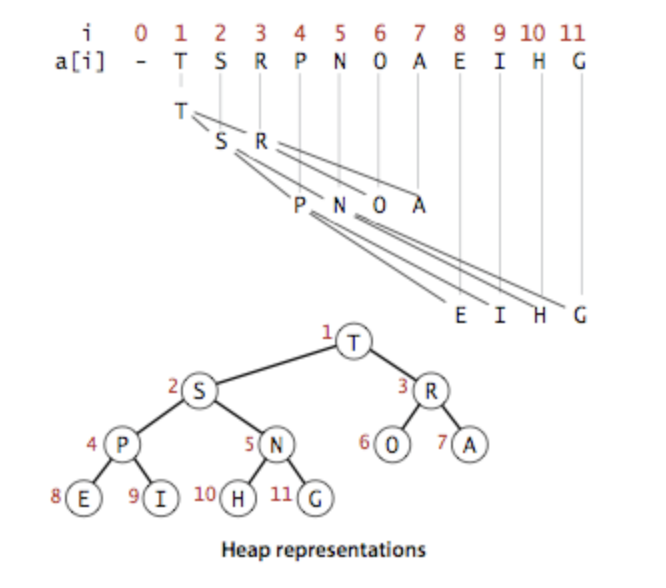
\includegraphics{Images/Heap.png}
  \label{fig:Heap}
\end{figure}

\begin{figure}[!ht]
  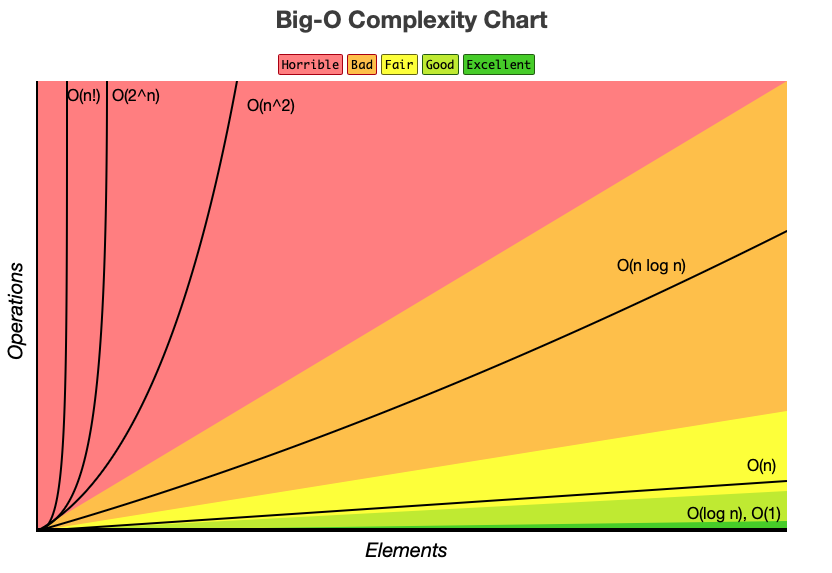
\includegraphics[width=\linewidth]{Images/BigO_Chart.png}
  \label{fig:Chart}
\end{figure}

\begin{figure}[!ht]
  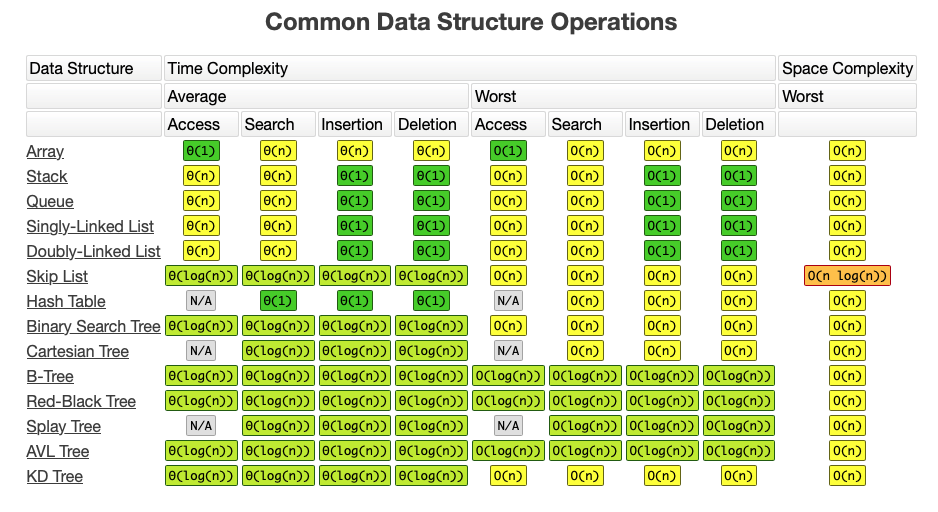
\includegraphics[width=\linewidth]{Images/DataStrucOpt.png}
  \label{fig:Chart2}
\end{figure}

\begin{figure}[!ht]
  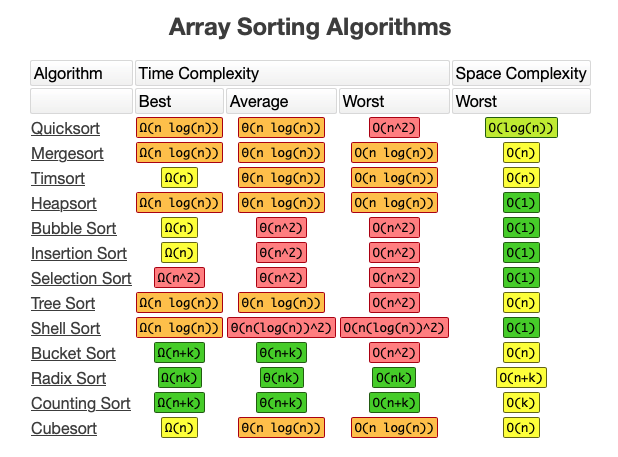
\includegraphics[width=\linewidth]{Images/ArraySortAlg.png}
  \label{fig:Chart3}
\end{figure}



\end{document}
 